\chapauthor{Никифоров С.А.\\Гойло А.А.}
\chapter{Языковые средства формального описания синтаксиса и денотационной семантики естественных языков в ostis-системах}
\chapauthortoc{Никифоров С.А.\\Гойло А.А.}
\label{chapter_lang}

\abstract{
    Аннотация к главе.

    Список доработок:
    \begin{textitemize}
        \item написать аннотацию;
        \item вставить отредактированный анализ из статьи (в частности, тут не нужно говорить про sem web и нужно убрать пару опасных высказываний, погорячился);
        \item формализовать все обобщенные правила,
        \item адекватное определения лексемы, пересмотреть термины для исклюения возможности появления омонимии / синонимии,
        \item примеры и пояснения,
        \item сказать что-то про отношения на лексемах,
        \item выделить пр. о. лексики,
        \item пройтись по подсказкам от плагина, поправит форматирование,
        \item формализовать пр. о..
    \end{textitemize}
    Список вопросов:
    \begin{textitemize}
        \item нужно ли фомрализвать все частные правила, их несколько десятков.
    \end{textitemize}
}

Проблема совместимости результатов исследований также остро стоит и в лингвистике -- науке, в которой существует множество различных теорий, часто несовместимых друг с другом.
В лингвистических исследованиях используются разные варианты разметки данных, нет одного подхода к структуризации корпусов текстов и различаются способы представления данных в них~\cite{Farrar2002ACO},~\cite{Chiarcos2012}.

В качестве решения проблемы несовместимости различных способов описания данных в лингвистике предлагались варианты стандартизации форматов такого описания.
Примером могут служить Text Encoding Initiative -- консорциум по стандартизации представления текстов в цифровом виде~\cite{Text_Encoding_Initiative} и гайдлайны экспертной группы по стандартизации представления языковых данных EAGLES (например, рекомендации по разметке корпусов текстов\cite{EAGLES_Recommendations}). Однако ни один из таких стандартов не получил распространения и не стал использоваться лингвистами повсеместно~\cite[p.~4]{Ide2010WhatDI}.

Вместо создания рекомендаций по разметке языкового материала в качестве более эффективного средства решения указанных выше проблем предлагается создание онтологий~\cite{schalley_2019},~\cite{mccrae_2015}. Помимо того, что онтология верхнего уровня для предметной области языкознания может служить связующим звеном между различными лингвистическими теориями, она также представляет собой формализованное описание лингвистических концептов, представленное в удобном для компьютеров формате, что обусловливает ее применимость в системах, способных понимать аннотированные языковые данные, совершать интеллектуальный поиск по корпусам текстов, а также потенциально выполнять анализ существующих лингвистических исследований~\cite{Farrar2002ACO}.

В качестве такой онтологии ПрО лингвистики выступает The General Ontology of Linguistic Description (GOLD)~\cite{gold}.
В этой онтологии формализованы наиболее базовые категории и отношения, используемые в лингвистике, а сама онтология интегрирована с онтологией верхнего уровня Suggested Upper Merged Ontology (SUMO)~\cite{pease_2002_sumo}. Авторы GOLD пишут, что создавали онтологию в первую очередь для того, чтобы решить проблему интероперабельности данных лингвистической типологии и для того, чтобы с ее помощью экспертные системы могли обрабатывать научные данные по естественным языкам -- т.е. целью создателей онтологии не являлось непосредственно решение задач из области обработки текстов на естественном языке~\cite{farrar_2003} (с.4).

Онтологией естественных языков, нацеленной непосредственно на использование при решении задач по обработке ЕЯ, является Ontologies of Linguistic Annotation (OLiA)~\cite{chiarcos-2012-ontologies}. Основной идеей онтологии является обеспечение совместимости разметки языковых данных, полученных в результате выполненного компьютерными системами анализа текстов на естественном языке с соответствующими им лингвистическими концептами из онтологии -- в отличие от других лингвистических онтологий, OLiA предоставляет не только инвентарь концептов и отношений, но и необходимую спецификацию интеграции этих элементов с разметкой языковых данных (например, в корпусах).~\cite[p.~4]{chiarcos-2012-ontologies}.

При создании онтологий естественного языка, встает вопрос о статусе спецификации лингвистической информации в таких онтологиях. Дж. Бейтман выделяет три типа онтологий в зависимости от интегрированности естественно-языковой информации в онтологию~\cite{Bateman_1997}:
\begin{enumerate}
    \item онтологии, представляющие собой абстрактную семантико-концептуальную репрезентацию знаний о мире, которая используется непосредственно в качестве денотационной семантики для синтаксиса и лексики естественного языка;
    \item онтологии, в которых есть отдельная спецификация денотационной семантики естественного языка, которая служит интерфейсом между синтаксисом естественных языков и собственно концептуальной онтологией;
    \item онтологии, представляющие собой абстрактную спецификацию знаний о реальном мире вне зависимости от ограничений естественного языка
\end{enumerate}

Популярность в сфере обработки естественного языка приобрел второй тип онтологии~\cite[p.~8]{Bateman_1997}, так как он, в отличие от третьего подхода, который совсем не формализует лингвистическую информацию, позволяет специфицировать больше информации о естественных языках. Так, одна из самых популярных онтологий, используемых в системах для обработки естественного языка, the Generalized Upper Model~\cite{Bateman2002TheGU}, является онтологией второго типа~\cite{Bateman_1997}.
П. Буителар и др. подчеркивают, что всем формальным онтологиям необходима связь с языковой информацией для решения таких задач как выделение информации из ЕЯ-текстов, автоматизированное заполнение онтологий и генерации текста на естественном языке~\cite{Buitelaar_2009}.

Так как использование онтологий в NLP позволяет задать семантику получаемым в результате обработки естественного языка данным и потенциально повысить качество NLP-анализа, начинается переход к созданию движимых онтологиями систем обработки естественных языков~\cite{Kostareva2016UsingOM},~\cite{nevzorova_2019}.
Онтологии естественного языка активно применяются для генерации ЕЯ-текстов на основе некоторой онтологии предметной области~\cite{cimiano-etal-2013-exploiting},~\cite{Bouayad_2014}.

Онтологический подход также используется в системах естественно-языковых запросов для баз данных, в которых запрос на естественном языке транслируется в язык запросов по онтологиям конкретных предметных областей, конструкции которого затем транслируются в SQL для обеспечения взаимодействия с реляционными базами данных~\cite{saha_2016}.

Кроме того, спецификация лингвистической информации в виде онтологий помогает решать задачу автоматизированного создания онтологий на основе естественно-языковых текстов~\cite{SHAMSFARD200417}.

Создаются онтологии частных областей лингвистики: например, онтология пространственных выражений в естественных языках~\cite{BATEMAN20101027}, онтология темпоральных сущностей на основе естественного языка~\cite{Moens_1987}, онтологии конкретных естественных языков~\cite{Dobrov_2018}.
При использовании онтологий для обработки естественного языка необходимо "связать"{} концепты из онтологии с лексикой конкретного ЕЯ.
Для этого создаются различные расширения существующих языковых БД, таких как WordNet~\cite{wordnet}, VerbNet~\cite{verbnet} и FrameNet~\cite{framenet}, направленные на их использование совместно с онтологиями верхнего уровня (например,~\cite{pease_fellbaum_2010}).
Активные разработки идут в сфере создания онтологий словарного состава естественных языков, в результате которых появилось множество формализованных описаний лексики~\cite{matsukawa-yokota-1991-development},~\cite{calzolari_1991},~\cite{buitelaar2006linginfo},~\cite{Cimiano2007LexOntoAM},~\cite{buitelaar_2006}.
Так как распространенные базы данных лексики ЕЯ не являются онтологиями и не имеют достаточной степени формализации (например, WordNet), создаются онтологии, являющиеся своего рода "надстройкой"{} над такими базами данных, самой известной из которых является lemon~\cite{McCrae_2012}.

Многие из приведенных выше онтологий созданы с использованием технологии Semantic Web~\cite{sem_web}, который является внешней технологией по отношению к существующим решениям для обработки естественных языков, поэтому последним приходится обращаться к ней с помощью API и стандартизированных языков запросов (в частности, SPARQL)~\cite{Bouayad_2014}.

Стоит отметить, что несмотря на активное развитие в направлении применения онтологий для обработки ЕЯ, многие популярные NLP-библиотеки (например, NLTK~\cite{nltk} и spaCy~\cite{spacy}) в принципе не поддерживают использование онтологий, а большинство инструментов для разметки естественно-языковых текстов используют обычно свой формат, что требует использования специфичных для таких инструментов парсеров и конвертеров, чтобы данные можно было применить при решении каких-либо задач~\cite[p.~3]{Erekhinskaya2020TenWO}.

Таким образом, в настоящее время в данной области можно выделить следующие проблемы:
\begin{enumerate}
    \item Отсутствие унификации (стандартизации) приведенных выше решений приводит к существенным накладным расходам на их интеграцию и значительно усложняет построение различных систем с их использованием в силу большой трудоемкости их интеграции~\cite{Standard2021},\cite{GolenkovProblems2021}.
    \item Несмотря на то, что онтологии потенциально способствуют решению широкого круга задач в сфере обработки естественного языка, большинство движимых онтологиями NLP-систем сконцентрированы на решении специализированных задач (например, только генерации текста, только заполнения онтологии или только обеспечения поиска с помощью естественного языка).
    \item Создано довольно большое количество частных лингвистических онтологий, формализующих, однако, лишь некий подраздел предметной области лингвистики (в особенности лексики), что отчасти вытекает из предыдущего пункта. В то же время, существующие лингвистические онтологии верхнего уровня (например, OLiA) все равно не до конца решают проблему унификации, т.к. им требуется вводить промежуточный уровень для интеграции полученных в результате NLP-анализа данных с фрагментами онтологии.
\end{enumerate}

Так как используемый в технологии OSTIS язык -- sc-код -- обладает достаточной экспрессивностью для описания знаний любого вида, а сама технология нацелена на создание интероперабельных интеллектуальных систем нового поколения, естественно-языковые интерфейсы ostis-систем смогут справляться с широким кругом задач по обработке текстов на естественных языках -- будь то синтез естественно-языковых текстов в целом, ведение диалога в диалоговых системах, поиск с использованием естественного языка, выделение информации из текстов и т.п. При этом в то время как в текущем состоянии сферы обработки естественных языков данные классы задач выполняются зачастую специализированными средствами и требуют дополнительных затрат на обеспечение потенциальной совместимости с конкретными компьютерными системами, в рамках технологии OSTIS для их решения будет использоваться один универсальный язык смыслового представления знаний, на котором будут написаны как компоненты решателя задач, так и онтология языков и конкретных предметных областей, что позволит решить проблему интероперабельности.

Более того, онтология естественных языков, разработанная в рамках такой технологии, могла бы быть использована не только для решения прикладных задач по обработке естественного языка, но и для обеспечения интероперабельности данных, полученных в ходе лингвистических исследований, что было бы ценным вкладом в область теоретической лингвистики.

Наконец, онтологию естественных языков можно рассматривать в качестве подмножества онтологии языков вообще (как естественных, так и искусственных и формальных), чего не делают рассмотренные выше существующие онтологии. Это позволит концептуализировать естественный язык в одной системе с языками программирования и более тесно связать используемые в соответствующих предметных областях понятия для более эффективного решения задач по обработке естественного языка в интеллектуальных компьютерных системах.

Цель данной работы -- предложить базовые средства формального описания синтаксиса и денотационной семантики различных языков в виде фрагмента онтологии языков и информационных конструкций, который можно будет использовать при проектировании интеллектуальных компьютерных систем нового поколения.
%Конец анализа

\section{Формализация естественных языков}

Как уже говорилось выше, для использования достижений лингвистики при проектировании интеллектуальных компьютерных систем требуется представить полученные результаты в формальном виде. В данном разделе мы предложим формализацию основных лингвистических концептов, выполненную на формальном языке представления знаний -- sc-коде.

\begin{SCn}

    \scnheader{язык}
    \begin{scnrelfromset}{разбиение}
        \scnitem{естественный язык}
        \begin{scnindent}
            \scntext{пояснение}{Естественный язык представляет собой язык, который не был создан целенаправленно}
        \end{scnindent}
        \scnitem{искусственный язык}
        \begin{scnindent}
            \scntext{пояснение}{Искусственный язык представляет собой язык, специально разработанный для достижения определённых целей}
            \scnhaselement{Эсперанто}
            \scnhaselement{Python}
            \scnsuperset{сконструированный язык}
            \begin{scnindent}
                \scntext{пояснение}{Сконструированный язык представляет собой искусственный язык, предназначенный для общения людей}
                \scnhaselement{Эсперанто}
            \end{scnindent}
        \end{scnindent}
    \end{scnrelfromset}

    \scnsuperset{международный язык}
    \begin{scnindent}
        \scntext{пояснение}{Международный язык представляет собой естественный или искусственный язык, использующийся для общения людей из разных стран}
        \scnhaselement{Английский язык}
        \scnhaselement{Русский язык}
    \end{scnindent}

    \scnheader{плановый язык}
    \begin{scnreltoset}{пересечение}
        \scnitem{сконструированный язык}
        \scnitem{международный язык}
    \end{scnreltoset}

    \scnheader{язык общения}
    \begin{scnreltoset}{объединение}
        \scnitem{естественный язык}
        \scnitem{сконструированный язык}
    \end{scnreltoset}
    \scnhaselement{Английский язык}
    \scnhaselement{Русский язык}
    \scnhaselement{Эсперанто}
    \begin{scnreltoset}{объединение}
        \scnitem{корневой язык}
        \begin{scnindent}
            \scntext{пояснение}{Корневой язык представляет собой язык, для которого характерно полное отсутствие словоизменения и наличие грамматической значимости порядка слов, состоящих только из корня.}
            \scnhaselement{Английский язык}
        \end{scnindent}
        \scnitem{агглютинативный язык}
        \begin{scnindent}
            \scntext{пояснение}{Агглютинативный язык характеризуется развитой системой употребления суффиксов, приставок, добавляемых к неизменяемой основе слова, которые используются для выражения категорий числа, падежа, рода и др.}
            \scnhaselement{Английский язык}
        \end{scnindent}
        \scnitem{флективный язык}
        \begin{scnindent}
            \scntext{пояснение}{Для флективного языка характерно развитое употребление окончаний для выражения категорий рода, числа, падежа, сложная система склонения глаголов, чередование гласных в корне, а также строгое различение частей речи.}
            \scnhaselement{Русский язык}
        \end{scnindent}
        \scnitem{профлективный язык}
        \begin{scnindent}
            \scntext{пояснение}{Для профлективного языка характерны агглютинация (в случае именного словоизменения), флексия и чередование гласных (аблаут)(в случае глагольного словоизменения).}
        \end{scnindent}
    \end{scnreltoset}

\end{SCn}

\section{Формализация синтаксиса естественных языков}

Лексема -- минимальная единица языка, имеющая семантическую интерпретацию и обозначающая концепт, отражающий взгляд на мир некоторого языкового сообщества \scncite{glossary}.

Грамматическая категория -- система противопоставленных друг другу рядов грамматических форм с однородными значениями. В рамках нашей формализации предлагается представить грамматические категории как классы ролевых отношений, каждый из которых соответствует определенному грамматическому значению. Следует отметить, что приводится онтология основных грамматических категорий, часто встречающихся в естественных языках, а не всех возможных.

\begin{SCn}

    \scnheader{грамматическая категория}
    \scnhaselement{лицо}
    \begin{scnindent}
        \scnrelto{семейство подмножеств}{ролевое отношение}
        \scnhaselement{первое лицо\scnrolesign}
        \scnhaselement{второе лицо\scnrolesign}
        \scnhaselement{третье лицо\scnrolesign}
    \end{scnindent}
    \scnhaselement{число}
    \begin{scnindent}
        \scnrelto{семейство подмножеств}{ролевое отношение}
        \scnhaselement{единственное число\scnrolesign}
        \scnhaselement{множественное число\scnrolesign}
        \scnhaselement{двойственное число\scnrolesign}
        \scnhaselement{тройственное число\scnrolesign}
        \scnhaselement{паукальное число\scnrolesign}
    \end{scnindent}
    \scnhaselement{род}
    \begin{scnindent}
        \scnrelto{семейство подмножеств}{ролевое отношение}
        \scnhaselement{мужской род\scnrolesign}
        \scnhaselement{средний род\scnrolesign}
        \scnhaselement{женский род\scnrolesign}
    \end{scnindent}
    \scnhaselement{падеж}
    \begin{scnindent}
        \scnrelto{семейство подмножеств}{ролевое отношение}
        \scnhaselement{именительный падеж\scnrolesign}
        \scnhaselement{родительный падеж\scnrolesign}
        \scnhaselement{дательный падеж\scnrolesign}
        \scnhaselement{винительный падеж\scnrolesign}
        \scnhaselement{творительный падеж\scnrolesign}
        \scnhaselement{предложный падеж\scnrolesign}
        \scnhaselement{звательный падеж\scnrolesign}
        \scnhaselement{абсолютивный падеж\scnrolesign}
        \scnhaselement{эргативный падеж\scnrolesign}
    \end{scnindent}
    \scnhaselement{время}
    \begin{scnindent}
        \scnrelto{семейство подмножеств}{ролевое отношение}
        \scnhaselement{настоящее время\scnrolesign}
        \scnhaselement{прошедшее время\scnrolesign}
        \scnhaselement{будущее время\scnrolesign}
    \end{scnindent}
    \scnhaselement{наклонение}
    \begin{scnindent}
        \scnrelto{семейство подмножеств}{ролевое отношение}
        \scnhaselement{изъявительное наклонение\scnrolesign}
        \scnhaselement{повелительное наклонение\scnrolesign}
        \scnhaselement{сослагательное наклонение\scnrolesign}
        \scnhaselement{условное наклонение\scnrolesign}
    \end{scnindent}
    \scnhaselement{залог}
    \begin{scnindent}
        \scnrelto{семейство подмножеств}{ролевое отношение}
        \scnhaselement{действительный залог\scnrolesign}
        \scnhaselement{страдательный залог\scnrolesign}
        \scnhaselement{средний залог\scnrolesign}
        \scnhaselement{возвратный залог\scnrolesign}
        \scnhaselement{взаимный залог\scnrolesign}
    \end{scnindent}
    \scnhaselement{вид}
    \begin{scnindent}
        \scnrelto{семейство подмножеств}{ролевое отношение}
        \scnhaselement{совершенный вид\scnrolesign}
        \scnhaselement{несовершенный вид\scnrolesign}
        \scnhaselement{общий вид\scnrolesign}
        \scnhaselement{прогрессивный вид\scnrolesign}
        \scnhaselement{перфектный вид\scnrolesign}
    \end{scnindent}
    \scnhaselement{степень сравнения}
    \begin{scnindent}
        \scnrelto{семейство подмножеств}{ролевое отношение}
        \scnhaselement{положительная степень сравнения\scnrolesign}
        \scnhaselement{сравнительная степень сравнения\scnrolesign}
        \scnhaselement{превосходная степень сравнения\scnrolesign}
    \end{scnindent}
\end{SCn}

Пример формализации части приведенных выше отношений на языке sc.g приведен на рисунке~\ref{fig:lexeme_example}.

\begin{figure}[h]
    \centering
    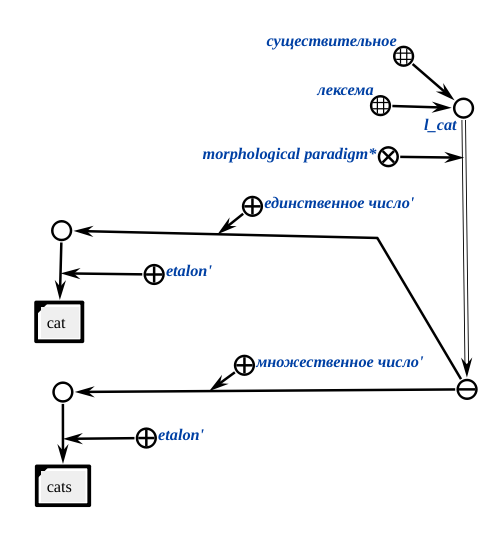
\includegraphics[width=0.4\textwidth]{images/part2/chapter_lang/lexeme_example.png}
    \caption{Пример спецификации лексемы в базе знаний.}
    \label{fig:lexeme_example}
\end{figure}

Часть речи -- категория, представляющая собой класс синтаксически эквивалентных знаков ЕЯ.

\begin{SCn}

    \scnheader{часть речи}
    \scnrelto{семейство подмножеств}{лексема}
    \scnhaselement{существительное}
    \scnhaselement{прилагательное}
    \scnhaselement{глагол}
    \scnhaselement{наречие}
    \scnhaselement{предлог}
    \scnhaselement{комплементатор}
    \scnhaselement{вспомогательный глагол}
    \scnhaselement{детерминант}

\end{SCn}

\textit{морфологическая парадигма*} - бинарное ориентированное отношение, связывающее лексему и множество ее словоформ.

Словоформа -- подмножество лексемы, которому принадлежат все вхождения лексемы с определенными грамматическими значениями. В рамках нашей онтологии словоформа понимается несколько иначе, чем принято в лингвистике, так как все вхождения лексемы в технологии OSTIS являются файлами.

При формализации синтаксиса в основном использовались стандартные положения генеративной грамматики \scncite{adger2003core}, \scncite{jackendoff1977x}, \scncite{haegeman1994introduction}, \scncite{carnie2012syntax}.

Дистрибуция знака –- это подмножество синтаксических правил, в которые входит данный знак.

Составляющая -- элемент множества C подмножеств кортежа вхождений лексем S, которое содержит в качестве элементов как сам S, так и все вхождения лексем в S, таким образом, что любые два подмножества, входящие в C, либо не пересекаются, либо одно из них включается в другое.

Непосредственно составляющая --  есть множество составляющих S, в которое входят составляющие A и B. В является непосредственно составляющей А если и только если В является подмножеством А и нет такой составляющей С, которая является подмножеством А и подмножеством которой является В.

Элементарная составляющая -- элемент кортежа вхождений лексем L, являющихся непосредственно составляющими множества составляющих C и не имеющих дочерних составляющих.

Синтаксическая группа -- класс составляющих, в который входят составляющие с вершинами, принадлежащими к одной части речи. Синтаксические группы представляют собой либо синглетон (минимально включают в себя вершину), либо упорядоченную пару, состояющую из вершины и другой синтаксической группы.

Вершина –- составляющая, дистрибуция которой совпадает с дистрибуцией всей синтаксической группы.

\begin{SCn}

    \scnheader{составляющая}
    \begin{scnrelfromset}{разбиение}
        \scnitem{синтаксическая группа}
        \scnitem{вершина}
    \end{scnrelfromset}

    \scnheader{синтаксическая группа}
% максимальная, промеж и вершины, вывести классы из примера как их пересечения
    \begin{scnrelfromset}{разбиение}
        \scnitem{именная группа}
        \begin{scnindent}
            \scntext{пояснение}{\textit{Именная группа} -- синтаксическая группа, вершиной которой является существительное.}
        \end{scnindent}
        \scnitem{глагольная группа}
        \begin{scnindent}
            \scntext{пояснение}{\textit{Глагольная группа} -- синтаксическая группа, вершиной которой является глагол.}
        \end{scnindent}
        \scnitem{группа прилагательного}
        \begin{scnindent}
            \scntext{пояснение}{\textit{Группа прилагательного} -- синтаксическая группа, вершиной которой является прилагательное.}
        \end{scnindent}
        \scnitem{наречная группа}
        \begin{scnindent}
            \scntext{пояснение}{\textit{Наречная группа} -- синтаксическая группа, вершиной которой является наречие.}
        \end{scnindent}
        \scnitem{предложная группа}
        \begin{scnindent}
            \scntext{пояснение}{\textit{Предложная группа} -- синтаксическая группа, вершиной которой является предлог.}
        \end{scnindent}
        \scnitem{группа комплементатора}
        \begin{scnindent}
            \scntext{пояснение}{\textit{Группа комплементатора} -- синтаксическая группа, вершиной которой является комплементатор.}
        \end{scnindent}
        \scnitem{временная группа}
        \begin{scnindent}
            \scntext{пояснение}{\textit{Временная группа} -- синтаксическая группа, вершиной которой является вспомогательный либо модальный глагол.}
        \end{scnindent}
        \scnitem{группа детерминанта}
        \begin{scnindent}
            \scntext{пояснение}{\textit{Группа детерминанта} -- синтаксическая группа, вершиной которой является детерминант.}
        \end{scnindent}
    \end{scnrelfromset}
    \begin{scnrelfromset}{разбиение}
        \scnitem{максимальная проекция вершины}
        \scnitem{промежуточная проекция вершины}
    \end{scnrelfromset}

\end{SCn}

При этом для упрощения могут быть введены более узкие классы, являющиеся пересечением приведенных выше, например \textit{максимальная проекция вершины группы детерминанта}.

\begin{SCn}

    \scnheader{максимальная проекция вершины группы детерминанта}
    \begin{scnreltoset}{пересечение}
        \scnitem{группа детерминанта}
        \scnitem{максимальная проекция вершины}
    \end{scnreltoset}

\end{SCn}

Пример синтаксической структуры предложения, записанный с применением введенных выше понятий представлен на рисунке~\ref{pic_tree}.

\begin{figure*}[h]
    \centering
    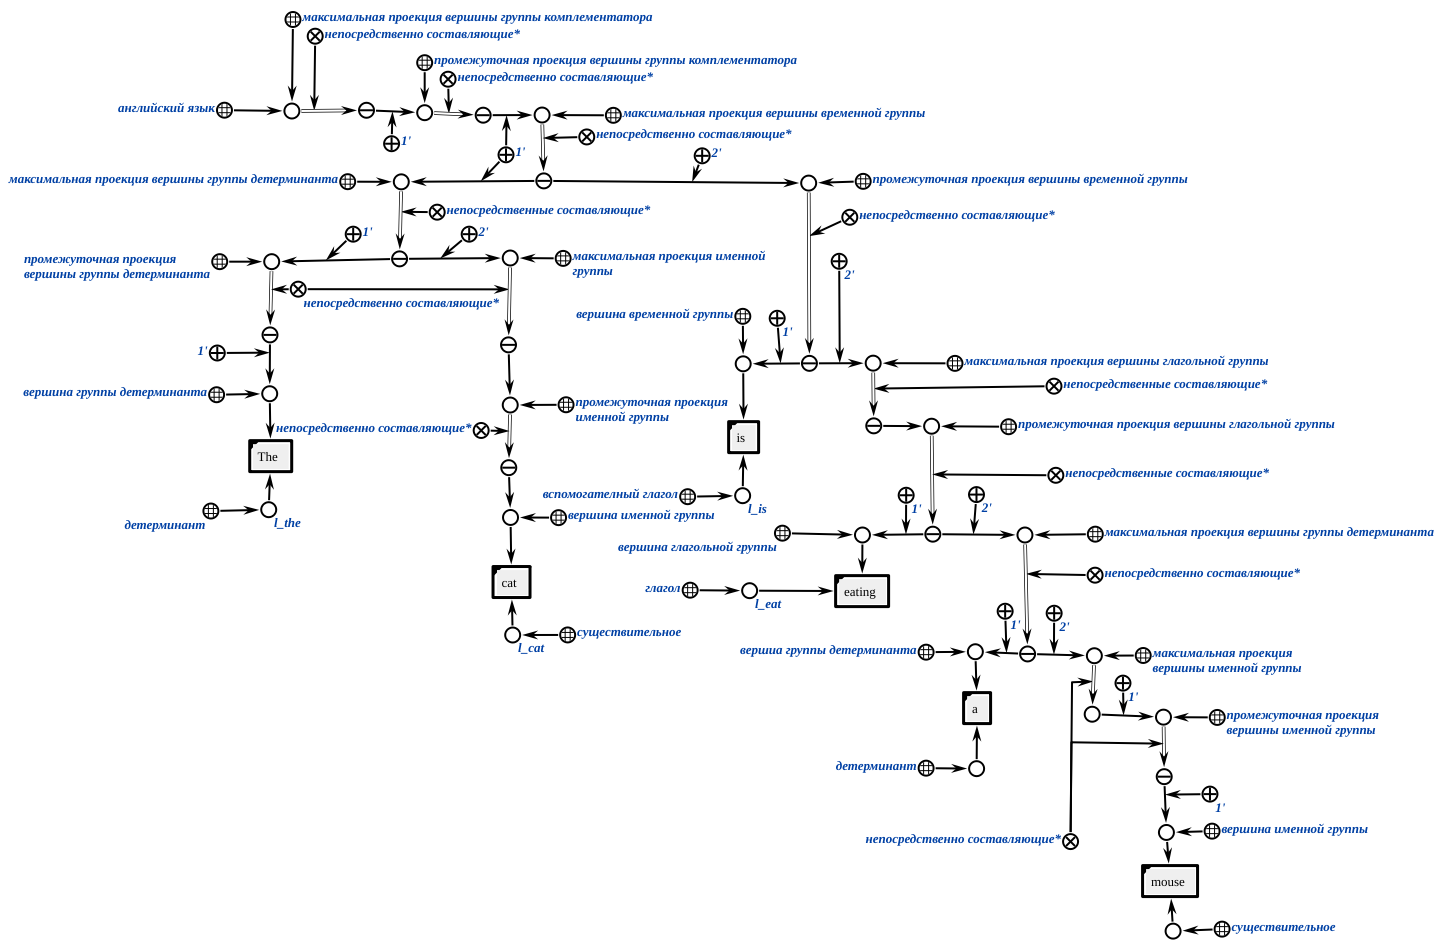
\includegraphics[width=\textwidth]{images/part2/chapter_lang/syntactic.png}
    \caption{Пример синтаксической структуры предложения.}
    \label{pic_tree}
\end{figure*}

Структуры синтаксических групп не являются произвольными -- элементы внутри группы могут граничить только с определенными множествами элементов.
Ниже приводятся возможные структуры синтаксических групп.
Знак "->"{} следует читать как "состоит из"{}.
В скобках указаны опциональные элементы.

Группа детерминанта:
\begin{textitemize}
    \item Максимальная проекция вершины группы детерминанта -> (Максимальная проекция вершины группы детерминанта) Промежуточная проекция вершины группы детерминанта
    \item Промежуточная проекция вершины группы детерминанта -> Вершина группы детерминанта (Максимальная проекция вершины именной группы)
\end{textitemize}

Именная группа:
\begin{textitemize}
    \item Максимальная проекция вершины именной группы -> (Максимальная проекция вершины группы детерминанта) Промежуточная проекция вершины именной группы
    \item Промежуточная проекция вершины именной группы -> (Максимальная проекция вершины группы прилагательного) Промежуточная проекция вершины именной группы ИЛИ Промежуточная проекция вершины именной группы (Максимальная проекция вершины предложной группы)
    \item Промежуточная проекция вершины именной группы -> Вершина именной группы (Максимальная проекция вершины предложной группы)
\end{textitemize}

Глагольная группа:
\begin{textitemize}
    \item Максимальная проекция вершины глагольной группы -> Промежуточная проекция вершины глагольной группы
    \item Промежуточная проекция вершины глагольной группы -> Промежуточная проекция вершины глагольной группы (Максимальная проекция вершины предложной группы) ИЛИ Промежуточная проекция вершины глагольной группы (Максимальная проекция вершины наречной группы)
    \item Промежуточная проекция вершины глагольной группы -> Вершина глагольной группы (Максимальная проекция вершины именной группы)
\end{textitemize}

Наречная группа:
\begin{textitemize}
    \item Максимальная проекция вершины наречной группы -> Промежуточная проекция вершины наречной группы
    \item Промежуточная проекция вершины наречной группы -> (Максимальная проекция вершины наречной группы) Промежуточная проекция вершины наречной группы
    \item Промежуточная проекция вершины наречной группы -> Вершина наречной группы (Максимальная проекция вершины предложной группы)
\end{textitemize}

Группа прилагательного:
\begin{textitemize}
    \item Максимальная проекция вершины группы прилагательного -> Промежуточная проекция вершины группы прилагательного
    \item Промежуточная проекция вершины группы прилагательного -> (Максимальная проекция вершины наречной группы) + Промежуточная проекция вершины группы прилагательного
    \item Промежуточная проекция вершины группы прилагательного -> Вершина группы прилагательного (Максимальная проекция вершины предложной группы)
\end{textitemize}

Предложная группа:
\begin{textitemize}
    \item Максимальная проекция вершины предложной группы -> Промежуточная проекция вершины предложной группы
    \item Промежуточная проекция вершины предложной группы -> Промежуточная проекция вершины предложной группы (Максимальная проекция вершины предложной группы) ИЛИ (Максимальная проекция вершины наречной группы) Промежуточная проекция вершины предложной группы
    \item Промежуточная проекция вершины предложной группы -> Вершина предложной группы (Максимальная проекция вершины именной группы)
\end{textitemize}

Временная группа:
\begin{textitemize}
    \item Максимальная проекция вершины временной группы -> (Максимальная проекция вершины группы детерминанта) Промежуточная проекция вершины временной группы
    \item Промежуточная проекция вершины временной группы -> Вершина временной группы (Максимальная проекция вершины глагольной группы)
\end{textitemize}

Группа комплементатора:
\begin{textitemize}
    \item Максимальная проекция вершины группы комплементатора -> (Максимальная проекция вершины некоторой синтаксической группы) Промежуточная проекция вершины группы комплементатора
    \item Промежуточная проекция вершины группы комплементатора -> Вершина группы комплементатора Максимальная проекция вершины временной группы
\end{textitemize}

В формальном виде данные правила можно представить следующим образом (см. рисунок~\ref{fig:pic_tree_structure_rule}).

\begin{figure*}[h]
    \centering
    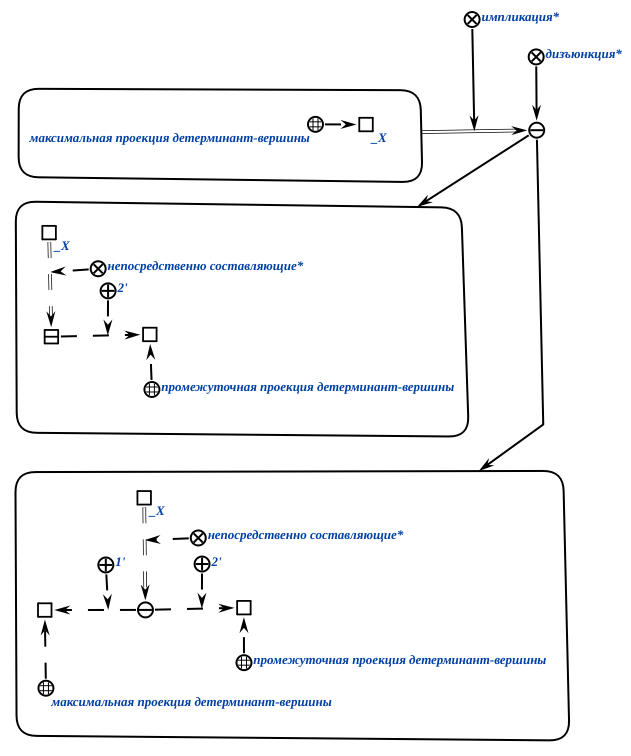
\includegraphics[width=0.8\textwidth]{images/part2/chapter_lang/tree_structure_rule.png}
    \caption{Пример правила структуры синтаксической группы.}
    \label{fig:pic_tree_structure_rule}
\end{figure*}

Комплемент -- синтаксическая группа, являющаяся сестрой вершины. Сестрами считаются составляющие, являющиеся непосредственно составляющими одной и той же составляющей.

Адъюнкт -- синтаксическая группа, являющаяся дочерью (непосредственно составляющей) промежуточной проекции и сестрой промежуточной проекции вершины той же синтаксической группы.

Спецификатор -- синтаксическая группа, являющейся дочерью максимальной проекции и сестрой промежуточной проекции.

Приведенные выше правила структуры синтаксических групп можно обобщить и свести к трем более абстрактным.

Правило спецификатора: XP -> (YP) X'

Правило адъюнкта: X' -> X' (ZP) | X' -> (ZP) X'

Правило комплемента: X' -> X (WP)

Формальное представление данных правил аналогично приведенному на рисунке~\ref{fig:pic_tree_structure_rule}.

\section{Формализация денотационной семантики естественных языков}

Денотационная семантика языка специфицирует интерпретацию элементов синтаксиса данного языка и представляет собой множество формул, описывающих то, каким образом знаковым конструкциям языка ставятся в соответствие обозначаемые ими сущности и конфигурации отношений между этими сущностями.

Денотационная семантика естественных языков должна обладать свойством композициональности -- т.е. интерпретация всего высказывания должна выводиться из интерпретации отдельных его частей. Таким образом, необходимо предоставить формальное описание интерпретации элементов синтаксиса ЕЯ, представленных в предыдущем разделе, а также описание правил совмещения интерпретации отдельных элементов для получения смысла всего высказывания.

В данной главе мы предлагаем вариант формализации денотационной семантики естественных языков в рамках технологии OSTIS, для составления которой использовались стандартные положения формальной семантики \scncite{heim1998semantics}, \scncite{Winter+2016}, \scncite{portner2008formal}.

Рассмотрим примеры правил, реализующих денотационную семантику языка. Приведенные ниже правила должны применяться последовательно и позволяют получить смысл текста естественного языка по его синтаксической структуре, "поднимаясь"{} по дереву составляющих от вершин к максимальным проекциям.

На рисунке~\textit{\nameref{fig:d_sem_1}} приведено правило, по которому происходит интерпретация вершин именной группы и группы прилагательного.
Смыслом таких вершин является класс, например: прилагательному "черный"{} соответствует множество черных объектов, а существительному "кот"{} -- множество котов.

\begin{figure}[H]
    \centering
    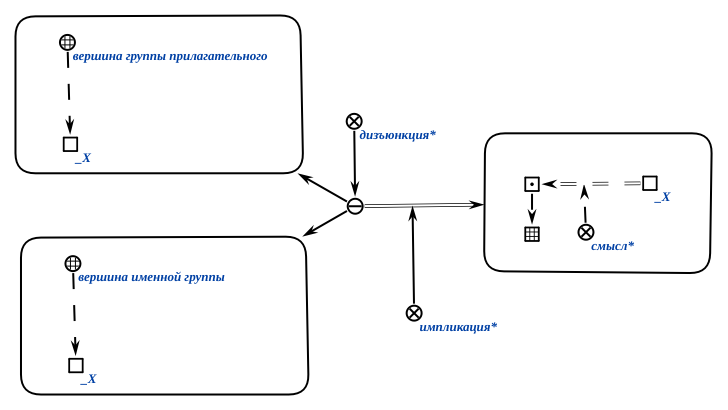
\includegraphics[width=0.8\textwidth]{images/part2/chapter_lang/d_sem_1}
    \caption{Правило интерпретации вершины группы прилагательного и вершины именной группы}
    \label{fig:d_sem_1}
\end{figure}
%в этом правиле мы интерпретируем вершины групп прилагательного и существительного - т.е. отдельные "слова"{}-прилагательные и существительные, которые у нас соответствуют классам

На рисунке~\textit{\nameref{fig:d_sem_2}} приведено правило, по которому происходит интерпретация именной группы, максимальная проекция которой включается в себя также группу прилагательного.
Как говорилось выше, для применения данного правила необходимо предварительное применение правила, представленного на рисунке~\textit{\nameref{fig:d_sem_1}}.
Смыслом таких конструкций является класс, являющийся результатом пересечения классов, полученных в результате интерпретации вершин групп прилагательного и именной группы по отдельности. Например: "черный кот"{} -- множество черных котов, пересечение множества котов и черных объектов. %ну все, теперь включаю мою кошку в соавторы

\begin{figure*}[h]
    \centering
    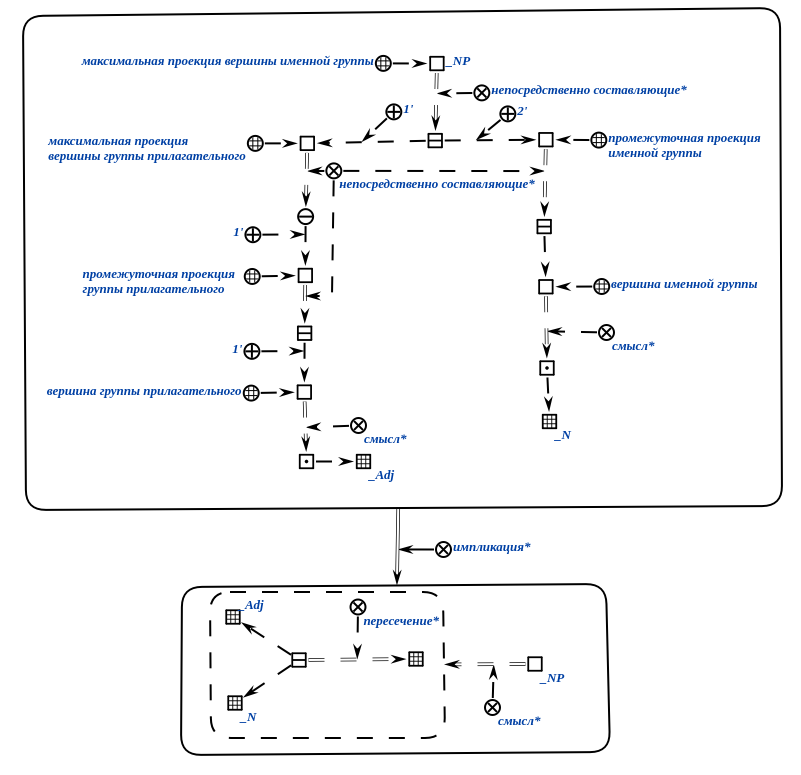
\includegraphics[width=0.8\textwidth]{images/part2/chapter_lang/d_sem_2.png}
    \caption{Правило интерпретации максимальной проекции вершины именной группы}
    \label{fig:d_sem_2}
\end{figure*}
%тут мы комбинируем смыслы прилагательного и существительного, которые входят в одну именную группу

На рисунке~\textit{\nameref{fig:d_sem_3}} приведено правило, по которому происходит интерпретация глагольной группы. Необходимость включения в посылку правила всей ветки глагольной группы объясняется ее необходимостью для определения типа глагола -- данное правило предназначено для интерпретации непереходных глаголов. Смыслом такой конструкции является класс действий.

\begin{figure*}[h]
    \centering
    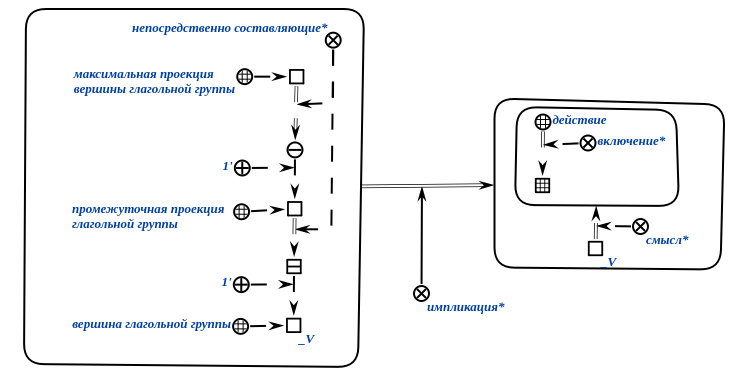
\includegraphics[width=0.8\textwidth]{images/part2/chapter_lang/d_sem_3.png}
    \caption{Правило интерпретации максимальной проекции вершины глагольной группы, содержащей непереходный глагол}
    \label{fig:d_sem_3}
\end{figure*}
%тут мы задаем интерпретацию всей глагольной группы (макс проекции) только для непереходных глаголов. написать, что смотрим по всей структуре группы целиком, потому что для того, чтобы отличить непереходный от переходного нам нужна вся ветка глагольной группы в дереве целиком

На рисунке~\textit{\nameref{d_sem_4}} приведено правило, по которому происходит интерпретация группы детерминанта с неопределенным артиклем. Смыслом такой конструкции является существование элемента класса, являющегося смыслом входящей в состав данной группы детерминанта именной группы.

\begin{figure*}[h]
    \centering
    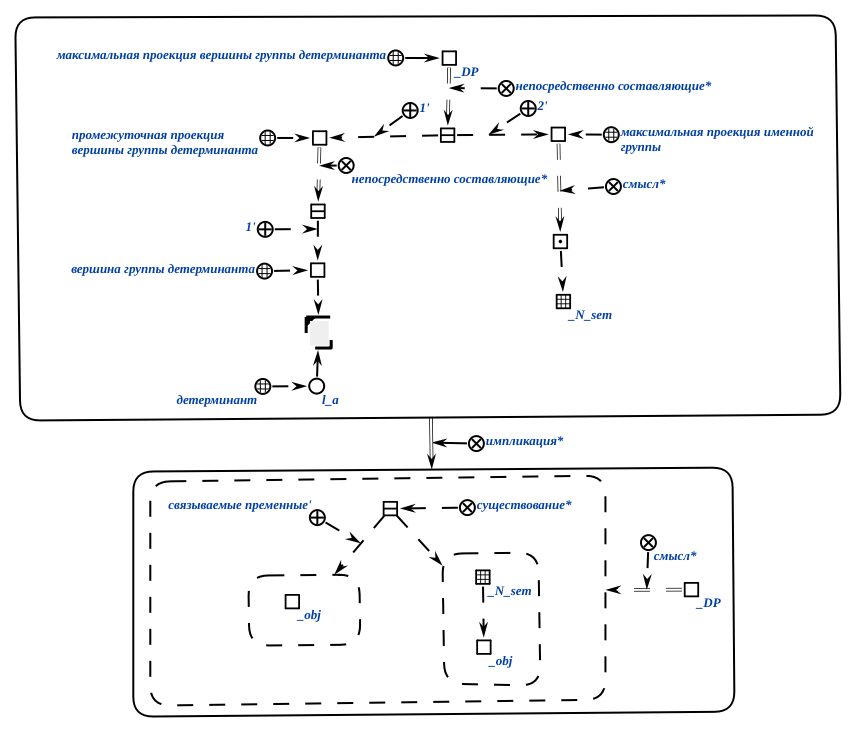
\includegraphics[width=0.8\textwidth]{images/part2/chapter_lang/d_sem_4.png}
    \caption{Правило интерпретации максимальной проекции вершины группы детерминанта}
    \label{d_sem_4}
\end{figure*}
%тут задается интерпретация сочетания именной группы с артиклем (в данном случае неопределенным)

На рисунке~\textit{\nameref{fig:d_sem_5}} приведено правило, по которому происходит интерпретация промежуточной проекции вершины временной группы, состоящей из вспомогательного глагола и полнозначного глагола. Вспомогательный глагол в данном случае задет класс действий по времени (является ли оно запланированным, выполняемым, уже выполненным и т.д.).

\begin{figure*}[h]
    \centering
    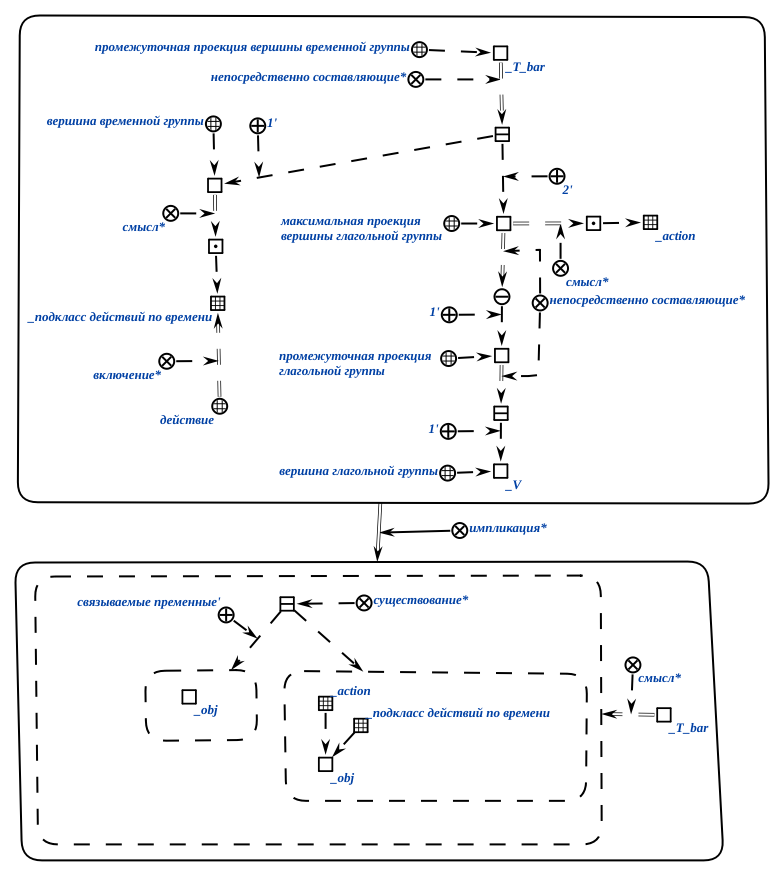
\includegraphics[width=0.8\textwidth]{images/part2/chapter_lang/d_sem_5.png}
    \caption{Правило интерпретации промежуточной проекции вершины временной группы}
    \label{fig:d_sem_5}
\end{figure*}
%тут задаем интерпретацию сочетания вспомогательного глагола и основного глагола. вспомогательный у нас соответствует классу действий по времени

На рисунке~\textit{\nameref{fig:d_sem_6}} приведено правило, по которому происходит интерпретация максимальной проекции вершины временной группы на основе полученного на предыдущем шаге смысла промежуточной проекции вершины временной группы и смысла максимальной проекции группы детерминанта.

\begin{figure*}[h]
    \centering
    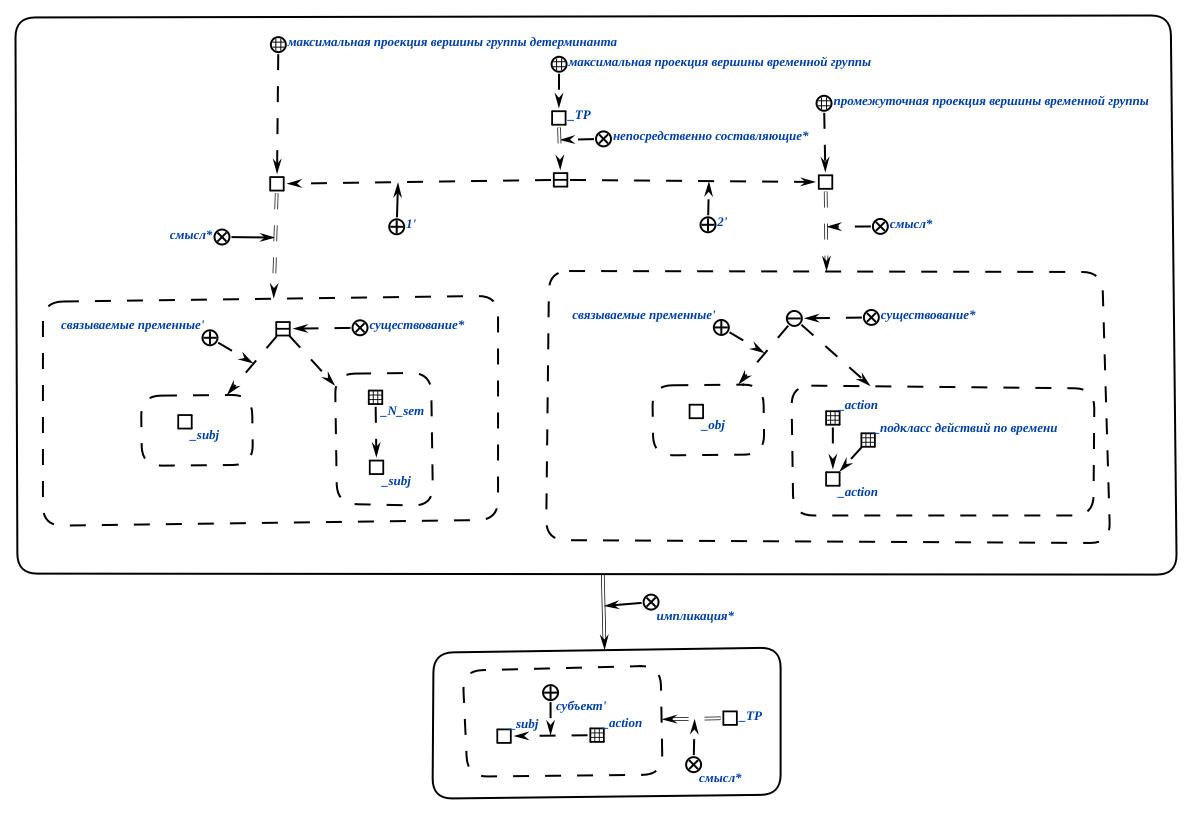
\includegraphics[width=0.8\textwidth]{images/part2/chapter_lang/d_sem_6.png}
    \caption{Правило интерпретации максимальной проекции вершины временной группы}
    \label{fig:d_sem_6}
\end{figure*}
%тут задаем интерпретацию для аргументной структуры непереходного глагола (сочетания подлежащего с непереходным глаголом)

На рисунке~\textit{\nameref{fig:d_sem_7}} приведено правило, по которому происходит интерпретация максимальной проекции вершины группы комплементатора на основе полученных на предыдущих шагах смыслов более частных конструкций. Данным правилом задается интерпретация предложения с переходным глаголом.

\begin{figure*}[h]
    \centering
    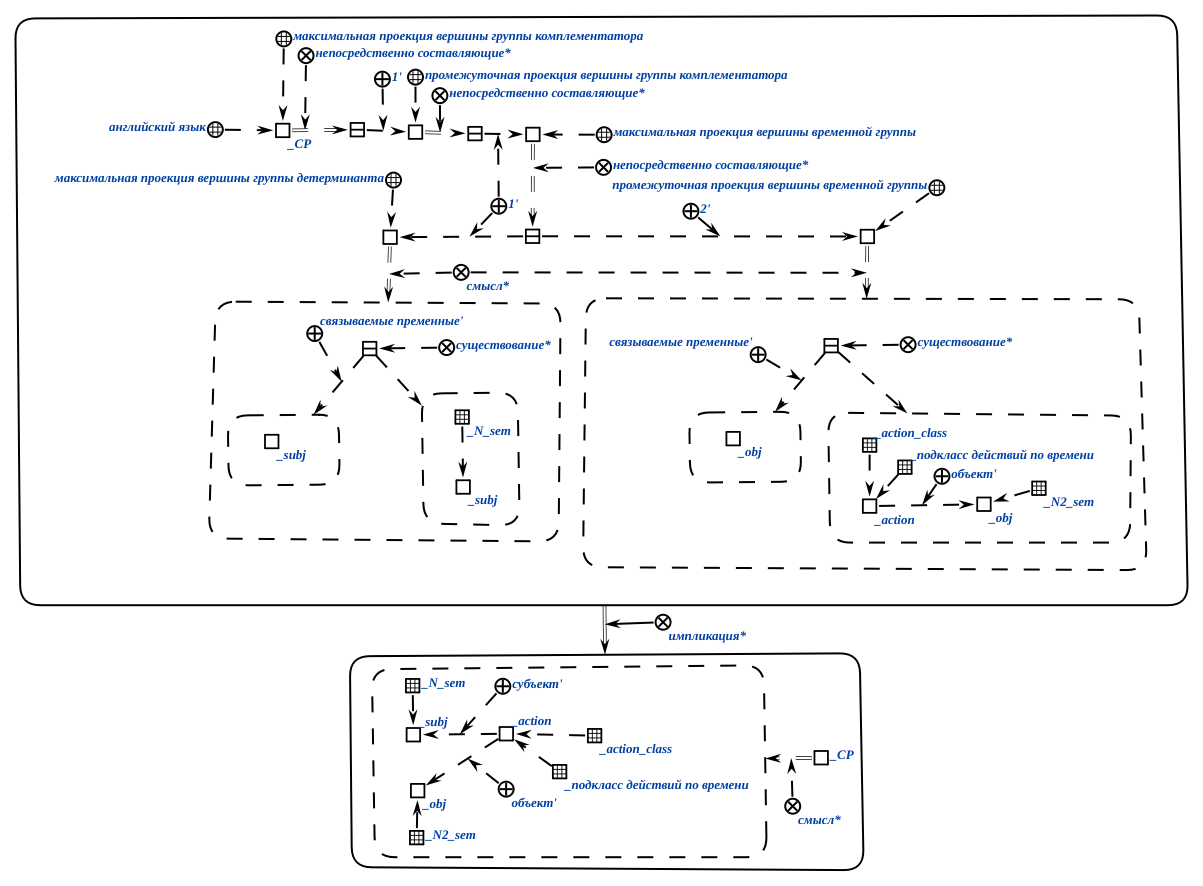
\includegraphics[width=0.8\textwidth]{images/part2/chapter_lang/d_sem_7.png}
    \caption{Правило интерпретации предложения с переходным глаголом}
    \label{fig:d_sem_7}
\end{figure*}
%тут задаем интерпретацию аргументной структуры переходного глагола (сочетания переходного глагола с его аргументами - подлажещим и дополнением)

%%%%%%%%%%%%%%%%%%%%%%%%% referenc.tex %%%%%%%%%%%%%%%%%%%%%%%%%%%%%%
% sample references
% %
% Use this file as a template for your own input.
%
%%%%%%%%%%%%%%%%%%%%%%%% Springer-Verlag %%%%%%%%%%%%%%%%%%%%%%%%%%
%
% BibTeX users please use
% \bibliographystyle{}
% \bibliography{}
%
\biblstarthook{In view of the parallel print and (chapter-wise) online publication of your book at \url{www.springerlink.com} it has been decided that -- as a genreral rule --  references should be sorted chapter-wise and placed at the end of the individual chapters. However, upon agreement with your contact at Springer you may list your references in a single seperate chapter at the end of your book. Deactivate the class option \texttt{sectrefs} and the \texttt{thebibliography} environment will be put out as a chapter of its own.\\\indent
References may be \textit{cited} in the text either by number (preferred) or by author/year.\footnote{Make sure that all references from the list are cited in the text. Those not cited should be moved to a separate \textit{Further Reading} section or chapter.} If the citatiion in the text is numbered, the reference list should be arranged in ascending order. If the citation in the text is author/year, the reference list should be \textit{sorted} alphabetically and if there are several works by the same author, the following order should be used:
\begin{enumerate}
\item all works by the author alone, ordered chronologically by year of publication
\item all works by the author with a coauthor, ordered alphabetically by coauthor
\item all works by the author with several coauthors, ordered chronologically by year of publication.
\end{enumerate}
The \textit{styling} of references\footnote{Always use the standard abbreviation of a journal's name according to the ISSN \textit{List of Title Word Abbreviations}, see \url{http://www.issn.org/en/node/344}} depends on the subject of your book:
\begin{itemize}
\item The \textit{two} recommended styles for references in books on \textit{mathematical, physical, statistical and computer sciences} are depicted in ~\cite{science-contrib, science-online, science-mono, science-journal, science-DOI} and ~\cite{phys-online, phys-mono, phys-journal, phys-DOI, phys-contrib}.
\item Examples of the most commonly used reference style in books on \textit{Psychology, Social Sciences} are~\cite{psysoc-mono, psysoc-online,psysoc-journal, psysoc-contrib, psysoc-DOI}.
\item Examples for references in books on \textit{Humanities, Linguistics, Philosophy} are~\cite{humlinphil-journal, humlinphil-contrib, humlinphil-mono, humlinphil-online, humlinphil-DOI}.
\item Examples of the basic Springer style used in publications on a wide range of subjects such as \textit{Computer Science, Economics, Engineering, Geosciences, Life Sciences, Medicine, Biomedicine} are ~\cite{basic-contrib, basic-online, basic-journal, basic-DOI, basic-mono}. 
\end{itemize}
}

\begin{thebibliography}{99.}%
% and use \bibitem to create references.
%
% Use the following syntax and markup for your references if 
% the subject of your book is from the field 
% "Mathematics, Physics, Statistics, Computer Science"
%
% Contribution 
\bibitem{science-contrib} Broy, M.: Software engineering --- from auxiliary to key technologies. In: Broy, M., Dener, E. (eds.) Software Pioneers, pp. 10-13. Springer, Heidelberg (2002)
%
% Online Document
\bibitem{science-online} Dod, J.: Effective substances. In: The Dictionary of Substances and Their Effects. Royal Society of Chemistry (1999) Available via DIALOG. \\
\url{http://www.rsc.org/dose/title of subordinate document. Cited 15 Jan 1999}
%
% Monograph
\bibitem{science-mono} Geddes, K.O., Czapor, S.R., Labahn, G.: Algorithms for Computer Algebra. Kluwer, Boston (1992) 
%
% Journal article
\bibitem{science-journal} Hamburger, C.: Quasimonotonicity, regularity and duality for nonlinear systems of partial differential equations. Ann. Mat. Pura. Appl. \textbf{169}, 321--354 (1995)
%
% Journal article by DOI
\bibitem{science-DOI} Slifka, M.K., Whitton, J.L.: Clinical implications of dysregulated cytokine production. J. Mol. Med. (2000) doi: 10.1007/s001090000086 
%
\bigskip

% Use the following (APS) syntax and markup for your references if 
% the subject of your book is from the field 
% "Mathematics, Physics, Statistics, Computer Science"
%
% Online Document
\bibitem{phys-online} J. Dod, in \textit{The Dictionary of Substances and Their Effects}, Royal Society of Chemistry. (Available via DIALOG, 1999), 
\url{http://www.rsc.org/dose/title of subordinate document. Cited 15 Jan 1999}
%
% Monograph
\bibitem{phys-mono} H. Ibach, H. L\"uth, \textit{Solid-State Physics}, 2nd edn. (Springer, New York, 1996), pp. 45-56 
%
% Journal article
\bibitem{phys-journal} S. Preuss, A. Demchuk Jr., M. Stuke, Appl. Phys. A \textbf{61}
%
% Journal article by DOI
\bibitem{phys-DOI} M.K. Slifka, J.L. Whitton, J. Mol. Med., doi: 10.1007/s001090000086
%
% Contribution 
\bibitem{phys-contrib} S.E. Smith, in \textit{Neuromuscular Junction}, ed. by E. Zaimis. Handbook of Experimental Pharmacology, vol 42 (Springer, Heidelberg, 1976), p. 593
%
\bigskip
%
% Use the following syntax and markup for your references if 
% the subject of your book is from the field 
% "Psychology, Social Sciences"
%
%
% Monograph
\bibitem{psysoc-mono} Calfee, R.~C., \& Valencia, R.~R. (1991). \textit{APA guide to preparing manuscripts for journal publication.} Washington, DC: American Psychological Association.
%
% Online Document
\bibitem{psysoc-online} Dod, J. (1999). Effective substances. In: The dictionary of substances and their effects. Royal Society of Chemistry. Available via DIALOG. \\
\url{http://www.rsc.org/dose/Effective substances.} Cited 15 Jan 1999.
%
% Journal article
\bibitem{psysoc-journal} Harris, M., Karper, E., Stacks, G., Hoffman, D., DeNiro, R., Cruz, P., et al. (2001). Writing labs and the Hollywood connection. \textit{J Film} Writing, 44(3), 213--245.
%
% Contribution 
\bibitem{psysoc-contrib} O'Neil, J.~M., \& Egan, J. (1992). Men's and women's gender role journeys: Metaphor for healing, transition, and transformation. In B.~R. Wainrig (Ed.), \textit{Gender issues across the life cycle} (pp. 107--123). New York: Springer.
%
% Journal article by DOI
\bibitem{psysoc-DOI}Kreger, M., Brindis, C.D., Manuel, D.M., Sassoubre, L. (2007). Lessons learned in systems change initiatives: benchmarks and indicators. \textit{American Journal of Community Psychology}, doi: 10.1007/s10464-007-9108-14.
%
%
% Use the following syntax and markup for your references if 
% the subject of your book is from the field 
% "Humanities, Linguistics, Philosophy"
%
\bigskip
%
% Journal article
\bibitem{humlinphil-journal} Alber John, Daniel C. O'Connell, and Sabine Kowal. 2002. Personal perspective in TV interviews. \textit{Pragmatics} 12:257--271
%
% Contribution 
\bibitem{humlinphil-contrib} Cameron, Deborah. 1997. Theoretical debates in feminist linguistics: Questions of sex and gender. In \textit{Gender and discourse}, ed. Ruth Wodak, 99--119. London: Sage Publications.
%
% Monograph
\bibitem{humlinphil-mono} Cameron, Deborah. 1985. \textit{Feminism and linguistic theory.} New York: St. Martin's Press.
%
% Online Document
\bibitem{humlinphil-online} Dod, Jake. 1999. Effective substances. In: The dictionary of substances and their effects. Royal Society of Chemistry. Available via DIALOG. \\
http://www.rsc.org/dose/title of subordinate document. Cited 15 Jan 1999
%
% Journal article by DOI
\bibitem{humlinphil-DOI} Suleiman, Camelia, Daniel C. O'Connell, and Sabine Kowal. 2002. `If you and I, if we, in this later day, lose that sacred fire...': Perspective in political interviews. \textit{Journal of Psycholinguistic Research}. doi: 10.1023/A:1015592129296.
%
%
%
\bigskip
%
%
% Use the following syntax and markup for your references if 
% the subject of your book is from the field 
% "Computer Science, Economics, Engineering, Geosciences, Life Sciences"
%
%
% Contribution 
\bibitem{basic-contrib} Brown B, Aaron M (2001) The politics of nature. In: Smith J (ed) The rise of modern genomics, 3rd edn. Wiley, New York 
%
% Online Document
\bibitem{basic-online} Dod J (1999) Effective Substances. In: The dictionary of substances and their effects. Royal Society of Chemistry. Available via DIALOG. \\
\url{http://www.rsc.org/dose/title of subordinate document. Cited 15 Jan 1999}
%
% Journal article by DOI
\bibitem{basic-DOI} Slifka MK, Whitton JL (2000) Clinical implications of dysregulated cytokine production. J Mol Med, doi: 10.1007/s001090000086
%
% Journal article
\bibitem{basic-journal} Smith J, Jones M Jr, Houghton L et al (1999) Future of health insurance. N Engl J Med 965:325--329
%
% Monograph
\bibitem{basic-mono} South J, Blass B (2001) The future of modern genomics. Blackwell, London 
%
\end{thebibliography}
